\documentclass[12pt]{article}
\usepackage{times}
\usepackage{amsmath}
\usepackage{enumerate}

\usepackage{hyperref}
\usepackage{graphicx,subfigure,latexsym,float}
\usepackage{fancyhdr}
\usepackage{alltt}
\usepackage{listing}
%%%%%\usepackage{draftwatermark}
%%%%%%\SetWatermarkFontSize{2.6cm}
%%%%%%\SetWatermarkText{DRAFT Evaluation Copy}
 
%set dimensions
\setlength{\textheight}{9.0in}
\setlength{\oddsidemargin}{0in}
\setlength{\evensidemargin}{0in}
\setlength{\topmargin}{0in}
\setlength{\textwidth}{6.5in}

\pagestyle{fancy}
\fancyhead[L]{}
\fancyhead[R]{}
\fancyhead[C]{}
\fancyfoot[L]{}
\fancyfoot[R]{}
\fancyfoot[C]{}

\fancyhead[L]{\slshape \rightmark}
\fancyhead[R]{\thepage}
%\fancyfoot[L]{\slshape \leftmark}

%\usepackage{pdfgraphcompat}    %% Put this before hyperref!!!!!
%\ifpdf
%  \usepackage[pdftex]{hyperref}
%\else
%\fi

\graphicspath{{./TechReportAndDocumentation_files/}}


\newcommand{\env}[1]{{\texttt{#1}}}
\newcommand{\fil}[1]{{\em #1}}
\newcommand{\cls}[1]{{\texttt{#1}}}
\newcommand{\sig}[1]{{\em #1}}
\newcommand{\pkg}[1]{{\texttt{#1}}}
\newcommand{\opt}[1]{{\em #1}}
\newcommand{\pgm}[1]{{\textbf{#1}}}
\newcommand{\dir}[1]{{\em #1}}
\newcommand{\sbr}[1]{{\em #1}}

\newcommand{\state}[1]{{\bf #1}}
\newcommand{\AND}{\bullet}
\newcommand{\nnp}{\newpage}
\newcommand{\nni}{\noindent}
\newcommand{\nnpi}{\newpage \noindent}

\newenvironment{codei}{\vspace{-0.1in} \begin{center} \begin{minipage}{6in} \noindent \begin{alltt}}{\end{alltt} \end{minipage} \end{center}}

\newenvironment{code}{\begin{center} \begin{minipage}{6in} \noindent \begin{alltt}}{\end{alltt} \end{minipage} \end{center}}

\makeatletter

\newcommand\problem{\@startsection{problem}{3}{\z@}%
                                     {-3.25ex\@plus -1ex \@minus -.2ex}%
                                     {1.5ex \@plus .2ex}%
                                     {\normalfont\normalsize\bfseries}}
\makeatother

\makeindex
\setcounter{tocdepth}{2}

\begin{document}

\floatstyle{ruled}
\newfloat{Program}{thp}{loa}[section]

\date{}
\title{{\bf \Huge \sc{RAPIDSMITH 2}}\\[0.1in]
%\hline\\[0.1in]
A Library for Low-level Manipulation 
of Vivado Designs at the Cell/BEL Level\\[0.3in]
%\hline\\[0.4in]
Technical Report and Documentation\\[0.1in]
}
\author{\Large Brent Nelson, Travis Haroldsen, Thomas Townsend\\[0.2in] \large NSF Center for High Performance Reconfigurable Computing (CHREC)
\thanks{This work was supported in part by the I/UCRC program of the National
 Science Foundation, grant numbers 0801876 and 1265957.}\\
\large Department of Electrical and Computer Engineering  \\
\large  Brigham Young University \\
\large  Provo, UT, 84602 \\[0.7in]
\large Last Modified: \today \\[0.05in]
}


\maketitle
\begin{figure}[H]
\centering
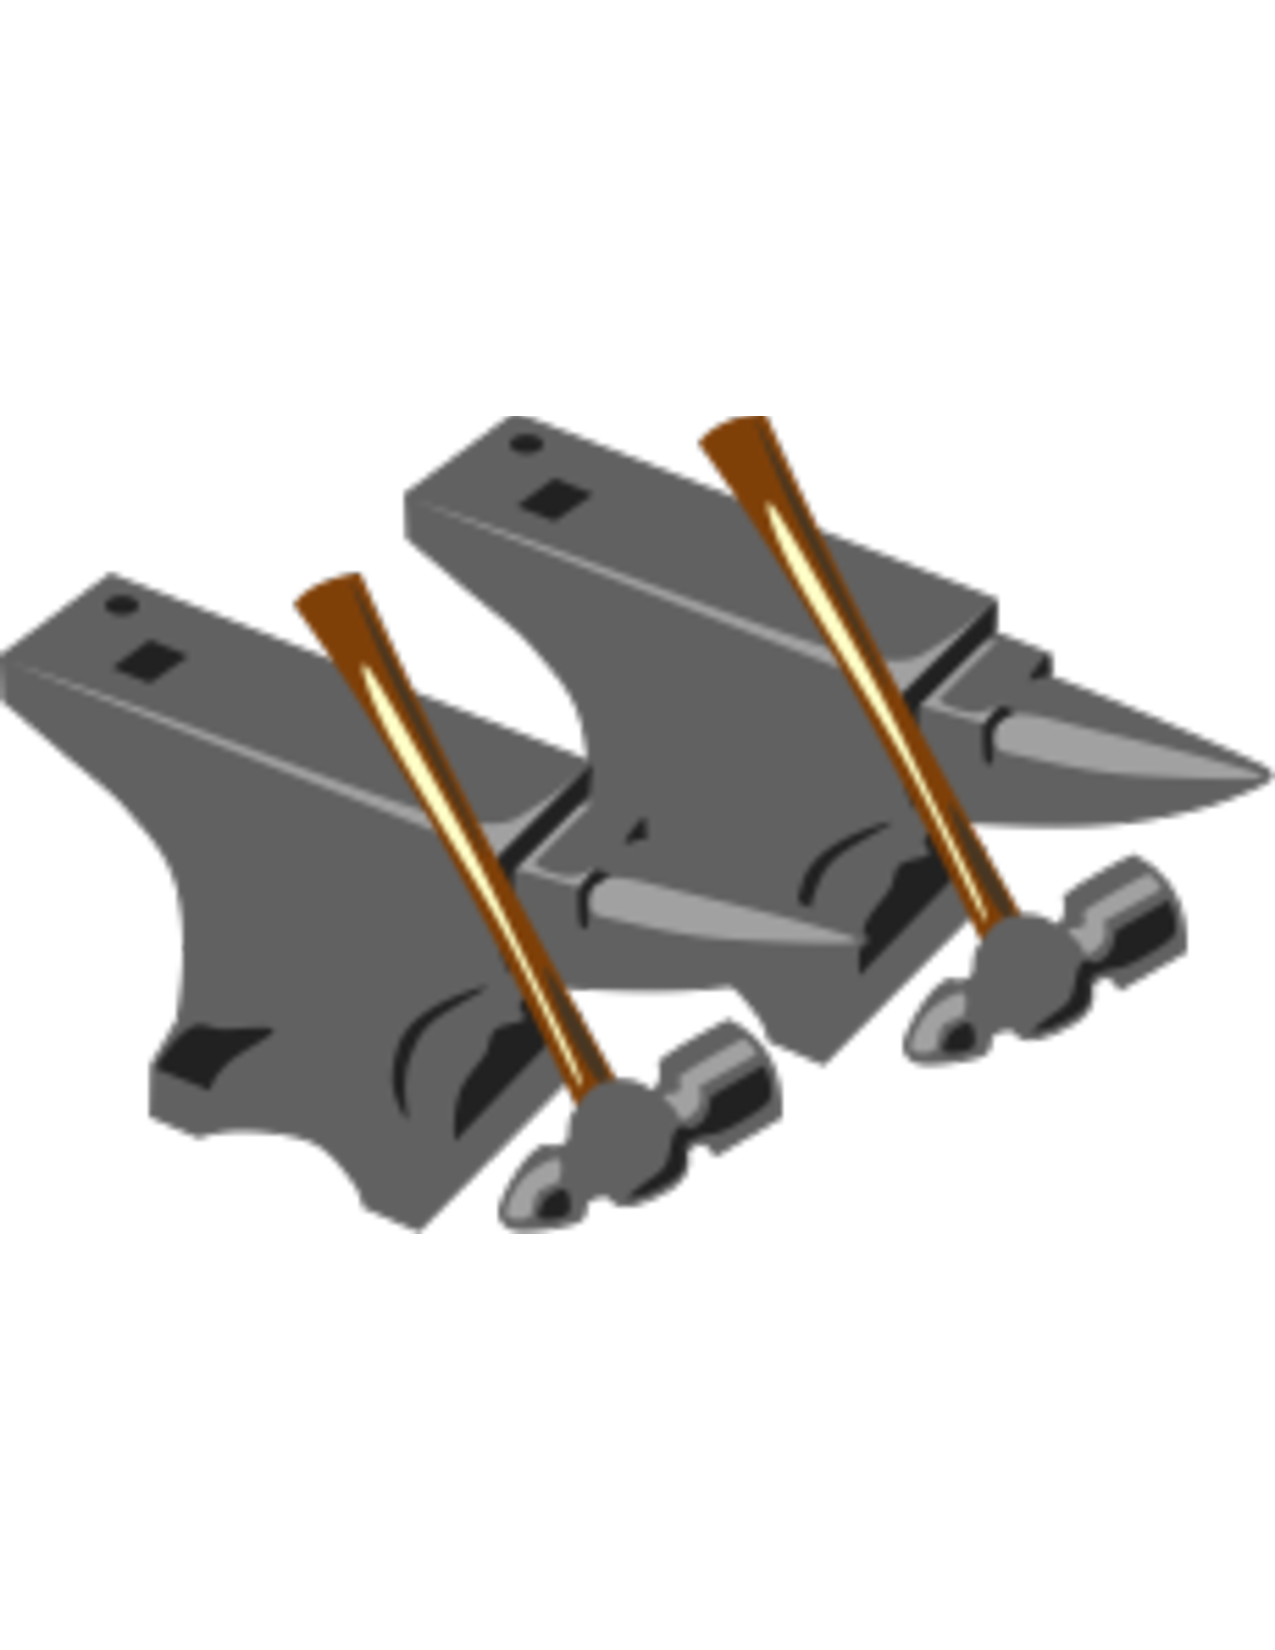
\includegraphics[width=0.4\columnwidth]{logo}
\end{figure}
\newpage
\tableofcontents
%\listoffigures


% \input{title}

\newpage
\section{Introduction}
\subsection{What is RapidSmith 2?}
The original BYU RapidSmith project began in 2010 with the goal to develop
a set of tools and APIs written in Java which would provide academics with an
easy-to-use platform to try out experimental CAD ideas and algorithms on modern
Xilinx FPGAs.  RapidSmith 2 (abbreviated RS2 hereafter) represents a major
addition to RapidSmith.  Using RS2 you can write custom CAD tools which will:
\begin{itemize}
  \item export designs from Vivado
  \item perform analyses on those designs
  \item make modifications to those designs
  \item import those designs back into Vivado for further processing or bitstream generation
\end{itemize}
In addition, you need not start with a Vivado design --- 
you can create a new
design from scratch in RS2 and then
import it into Vivado.

So, clearly a major addition with RS2 is the ability to work with Vivado. 
However, the other major new capability which RS2 adds over RapidSmith is that
it changes RapidSmith's design representation from the Instances and Sites of
ISE's XDL representation to the Cells and BELs of Vivado.   This is a
significant change as it exposes the actual design and device in a way that RapidSmith never
did, opening up new CAD research opportunities which were difficult
to perform using Rapidsmith.
       
\subsection{Who Should Use RS2?}
RS2 is aimed at anyone desiring to do FPGA CAD research on real Xilinx devices. 
It is written in Java. It also depends on some understanding of Xilinx FPGAs,
Vivado, and TCL.  However, the goal is that this documentation provides
sufficient background and detail to help bring developers up to speed on the
needed topics.    

RS2 by no means is a Xilinx Vivado replacement and cannot be used without a
valid and current license to a Xilinx tools installation (RS2 cannot generate
bitstreams for a design, for example).     

\subsection{Why RS2?}
The Xilinx-provided TCL interface into Vivado, in theory, provides all that is
needed to create any kind of CAD tool desired to augment the capabilities
provided by Vivado.  In practice there are a number of problems with that.
First, TCL is slow --- far too slow to execute a router for example.  Also the
Xilinx TCL interface does not manage memory well.  In our experience,
long-running scripts eventually cause the system to run out of memory. 
Brad White's MS work also determined
that not 100\% of the device information required to do arbitrary CAD
manipulations is available through TCL.  As a result, additional tools (and
some small amount of manual work) are required to provide the user (and CAD
tools they might like to write) with all the physical details on Xilinx parts.
Simply put, some information is not available through the TCL interface. 
Finally, the ability to export and import designs to/from Vivado and operate
on them outside Vivado using a modern high-level language such as Java is a
hugely useful capability.

RS2 (in conjunction with Tincr which is described in a later section of this
document) takes care of all of the generation of the FPGA part information that
is required by CAD tools. It also takes care of exporting/importing designs from
and to Vivado along with a myriad number of fairly arcane details associated
with that process.  In addition, RS2 creates special device files from the XDLRC
files produced by Tincr and provides a nice API into those physical device
details.  All of this enables researchers to have more time to focus on what
matters most: their research of new ideas and algorithms.

\subsection{Which Xilinx Parts does RS2 Support?}
As of the writing of this document, Artix 7 has been tested the most and is
currently supported in all forms and applications.  In addition, an Ultrascale
device file was created and demonstrated as a part of Brad White's MS work to
show that it is possible.  At some point, Ultrascale should be fully supported.
\footnote{An XDL-based import/export capability has also been created and used
with Virtex 6 devices as a part of Travis Haroldsen's PhD work but that path is
not being released, documented, or supported.}

As will be seen later, to generate additional device files for additional parts
within a supported family is relatively straightforward and can be done by any
user.  New families can also be supported but this
requires a bit more work.  As time goes on the process will become simpler ---
that is one of the goals for RS2 moving forward.

\subsection{How is RS2 Different than VPR and VTR?}
VPR (Versatile Place and Route) has been an FPGA research tool for several years
and has led to many publications on new FPGA CAD research.  It has been a
significant contribution to the FPGA research community and has grown to be a
complete FPGA CAD flow for research-based FPGAs.

The main difference between RapidSmith/RS2 and VPR is that the RapidSmith tools
aim to provide the ability to target commercial Xilinx FPGAs, providing the
ability to exit and re-enter the standard Xilinx flow at any point.  All
features of commercial FPGAs which are accessible via XDL and Vivado's TCL are available
in RapidSmith and RS2.  VPR currently is limited to FPGA features which can be
described using VPR's architectural description facilities.

\subsection{Why Java?}
We have found Java to be an excellent rapid prototyping platform for FPGA CAD
tools.  The Java libraries are rich with data structures useful for such
applications and Java eliminates the need to clean up objects in memory.  This
eliminates the time needed to debug such things, leaving more time for the
researcher to focus on the real research at hand.  Our experience over the past
decade is that for student research projects, the lack of memory management
problems (dangling pointers, memory leaks, …) and the associated errors has
greatly improved our student productivity and led to far more stable CAD tools.


\section{Vivado, RS2, and Tincr}
\subsection{RapidSmith vs. RS2}
\subsubsection{What Was The Original RapidSmith?}
The original RapidSmith was written by Christopher Lavin as a part of his PhD
work at BYU.  It was based on the Xilinx Design Language (XDL) which provides a
human-readable file format equivalent to the Xilinx proprietary Netlist Circuit
Description (NCD) of ISE.  With RapidSmith, researchers were able to import
XDL/NCD, manipulate, place, route and export designs among a variety of design
transformations.  The RapidSmith project made an excellent test bed to try out
new ideas and algorithms for FPGA CAD research because code could quickly be
written to take advantage of the APIs available.

RapidSmith also contained packages which could parse/export bitstreams (at the
packet level) and represent the frames and configuration blocks in the provided
data structures.  In this regard, RapidSmith did not include any proprietary
information about Xilinx FPGAs that is not publicly available.

RapidSmith continues to be functional and is still available at the
SourceForge.net website.  There, you will find documentation, installation
instructions, the RapidSmith code base, and a collection of demo programs based
on it.

\subsubsection{What is RS2?}
With the announced end of ISE (with the Virtex7 family of parts being the last
family to be supported by ISE), there was no path forward to newer parts using
RapidSmith.  This is because XDL is not available with Vivado. With
Vivado, however, Xilinx has provided an extensive TCL scripting capability which 
initially looked as if it could provide a similar capability to that provided by
XDL in terms of accessing both Vivado's design and device data and in terms of
creating and modifying Vivado designs.  However, as described above, Vivado's
Tcl is limited by speed and memory challenges.
The development of RS2 consisted of three parts.

\subsubsection{Tincr: Integrating Custom CAD Tool Frameworks with the Xilinx 
Vivado Design Suite} 

In the first part, the Vivado TCL capability was investigated to ensure that,
indeed, it did provide the needed ability to access design and device data and
export that to external tools such as RapidSmith.  This resulted in the Tincr
project, led by Brad White as a part of his MS work at BYU, with Thomas Townsend
making additions as a part of his research.

Tincr is a TCL-based library of routines which (a) provide a variety of
functions to simply make working with Vivado via TCL easier, (b) provide a way
to export all the data associated with a Vivado design into what is called a
Tincr Checkpoint (TCP), (c) provide a way to reimport Tincr Checkpoints back
into Vivado, and (d) access device data from Vivado and output that data in the
form of XDLRC files (these are the files which XDL used to describe devices and
are necessary for RapidSmith and RS2 to understand the structure of and the
resources available for use in a given Xilinx part).  Tincr is available at Github.com as
the project byuccl/Tincr.  Tincr is described in two publications:

\begin{quotation}B. White and B. Nelson, "Tincr — A custom CAD tool framework
for Vivado," 2014 International Conference on ReConFigurable Computing and FPGAs (ReConFig14),
Cancun, 2014, pp. 1-6, DOI: 10.1109/ReConFig.2014.7032560

White, Brad S., "Tincr: Integrating Custom CAD Tool Frameworks with
the Xilinx Vivado Design Suite" (2014), BYU Scholars Archive, Paper 4338. 
\\URL:http://scholarsarchive.byu.edu/etd/4338
\end{quotation}

\subsubsection{RS2: A Framework for BEL-Level CAD Exploration on Xilinx FPGAs}
The second part of the development of RS2 was to add a new layer of design
representation to RapidSmith which more closely matches that of Vivado.  This
was done as a part of his PhD work by Travis Haroldsen at BYU.  As of this
writing, one paper on RS2 has appeared:

\begin{quotation}Travis Haroldsen, Brent Nelson, and Brad Hutchings, “RapidSmith
2:
A Framework for BEL-Level CAD Exploration on Xilinx FPGAs�, Proceedings of the
2015 ACM/SIGDA International Symposium on Field-Programmable Gate Arrays,
February 2015, Monterey CA, pp. 66-69, DOI: 10.1145/2684746.2689085.
\end{quotation}

\subsubsection{Vivado and RS2 Integration}
The third part of the development of RS2 was to create the ability to export
designs from Vivado and into RS2 and, correspondingly, to import RS2 data back
into Vivado.  This was completed during 2016, largely by Thomas Townsend
as an MS student at Brigham Young University.  The initial
public release of RS2 was made in January 2017 once that piece was in place.

\subsubsection{What is All This About XDL and XDLRC and How Does RS2 Fit Into
That?} 
The Xilinx ISE tools had the capability to export XDL and XDLRC files which
RapidSmith used: 
\begin{itemize}
  \item An XDLRC file was a complete description of a given Xilinx FPGA,
  describing every tile, every switchbox, every wire segment, and every PIP in
  the part.  RapidSmith was able to process this information and create a device
  representation for use in support of CAD tools such as placers and routers.
  \item An XDL file was a textual representation of an NCD file (a user design).
  It described the user design as a collection of \cls{Instances} and \cls{Nets}. Instances
  correspond to things like {SLICEs}, {BRAMs}, {DSP48s}, and {IOBs}.  Instances could be
  placed onto \cls{Sites}. Additionally, Nets in XDL consisted of a list of
  \cls{Pins} (their logical connections) and an optional list of \cls{PIPs} (their physical
  routing connections).
\end{itemize}
In Vivado, however, designs are described as a collection of \cls{Cells} where a Cell
corresponds to things like LUTs, flip flops, etc.  A Cell may be placed
onto a \cls{BEL} object such as an ALUT or a BFF.  RS2 contains a new layer of
hierarchy in its design and device descriptions where Cells and BELs are first-class objects and
design manipulation is all done at the Cell/BEL level.

Also, Vivado Nets are described using directed routing strings rather than lists
of PIPs.  RS2 also contains a set of new classes to enable the representation
and manipulation of Nets in a format compatible with these routing strings.

Thus, using RS2, design manipulation is now done at the level of Cells and BELs
and importing/exporting designs to/from Vivado is now fully supported.

\subsection{RS2 Usage Model and Structure}
The usage model for RS2 is shown in \autoref{fig:UsageModels}.  As can be
seen, a design can be exported from Vivado at multiple different points in the
Vivado design flow.  In each case, Tincr is used to export a Tincr Checkpoint
which can then be imported into RS2.  At those same points in the design flow,
RS2 can export a Tincr Checkpoint which can then be imported back into Vivado. 
Thus, a complete solution involves Vivado, Tincr, and RS2.

\begin{figure}[htb]
\centering
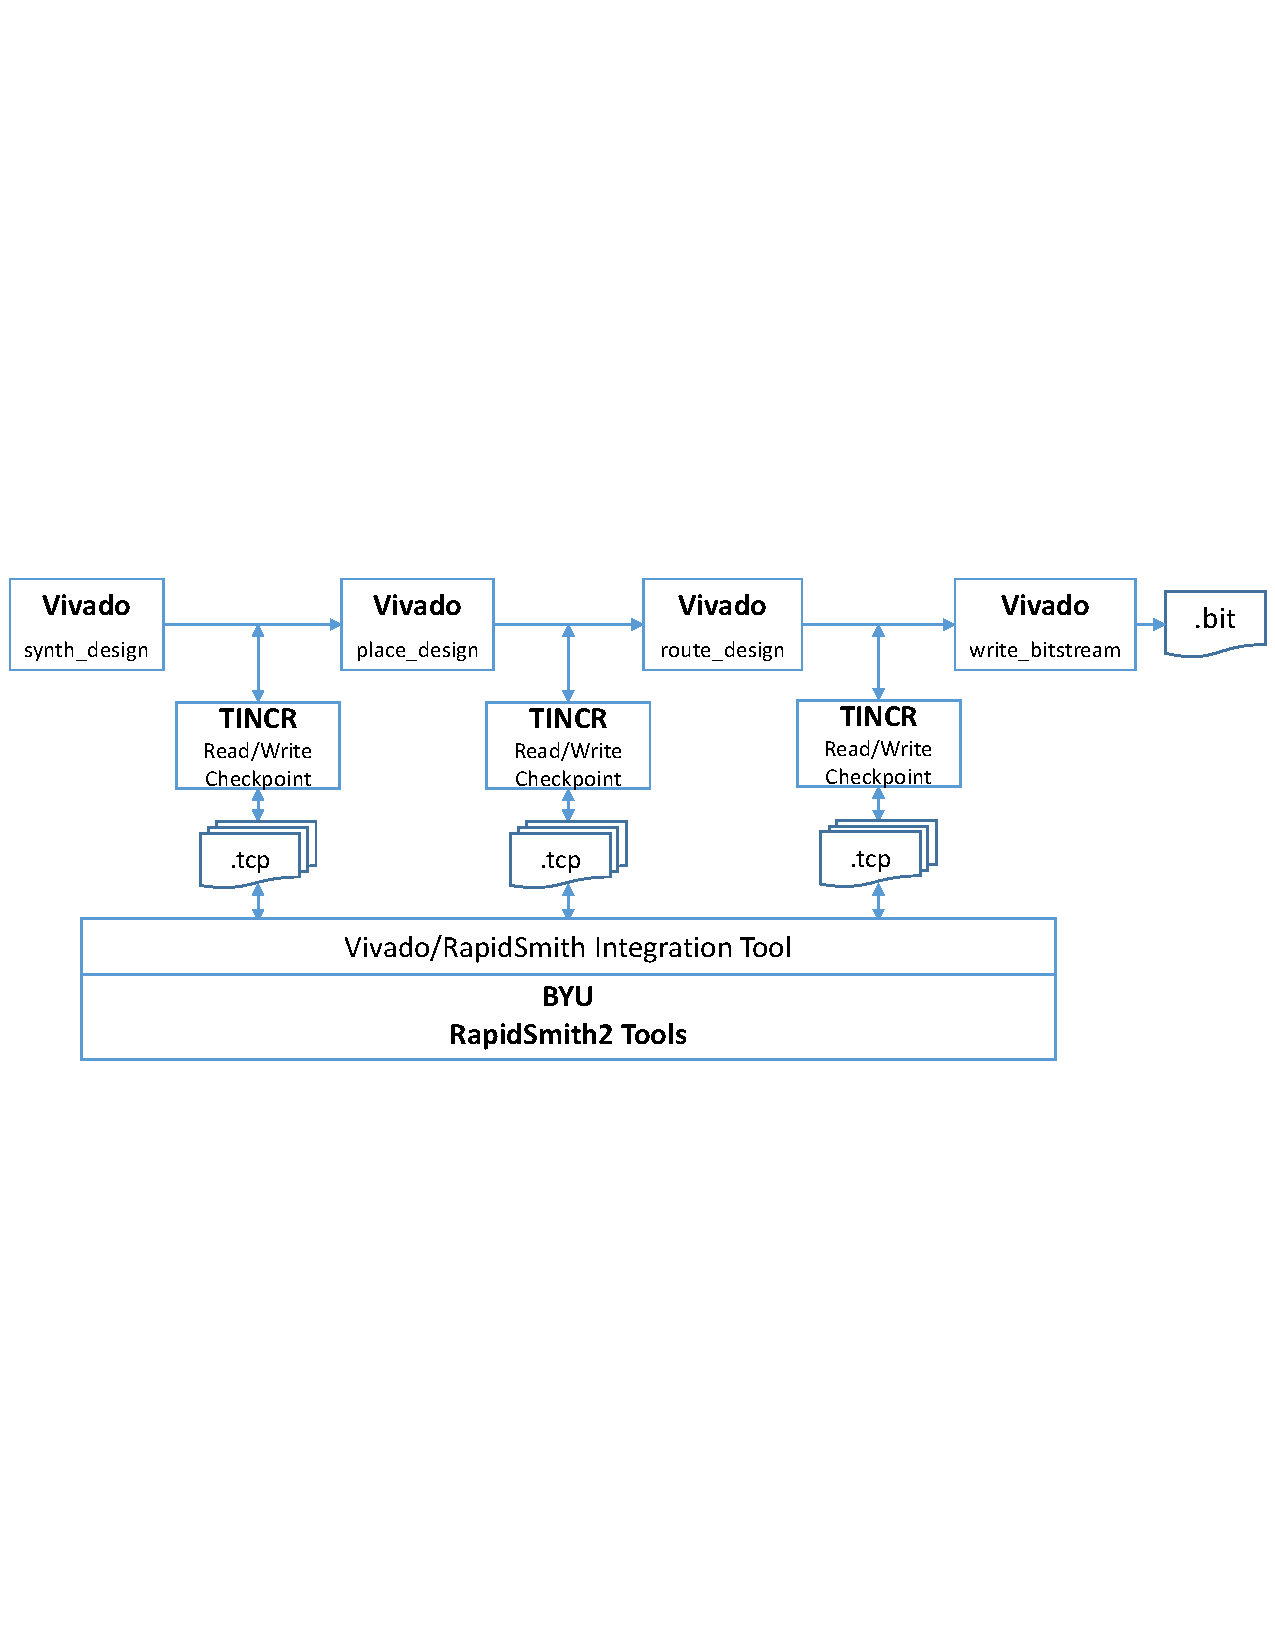
\includegraphics[width=\columnwidth]{UsageModels}
\caption{Vivado and RS2 Usage Model}
\label{fig:UsageModels}
\end{figure} 

\section{Getting Started}

\subsection{Installation}

RS2 is available on Github at: \url{https://github.com/byuccl/RapidSmith2}.  
You can either build RS2 into .class and .jar files for use in any Java
environment, or you can easily build RS2 for use in Eclipse (recommended).

\subsubsection{Requirements for Installation and Use}
\begin{itemize}
  \item Windows, Linux or Mac OS X all will work (see additional notes below for
  Mac OS X)
  \item Vivado
  \item JDK 1.8 or later
  \item Tincr 
\end{itemize}

Tincr is a companion project (\url{https://github.com/byuccl/tincr}) which 
is used for importing/exporting designs between Vivado
and RS2.  For getting started (running the example programs on the
provided sample designs) you will not need it installed.
Later, as you  actually start processing your own Vivado designs you will need
to obtain and install it.  

There are additional dependencies beyond these required for installation but
they are either provided in the distribution itself or are
automatically retrieved for you as a part of the installation process. 
Examples of these additional dependencies include QT Jambi, the BYU Edif Tools,
etc.
 
\subsubsection{Steps for Installation For Command Line Usage}
The first task is to acquire RS2 using git.
You can acquire the RS2 distribution by executing the following: 
\vspace{-0.15in}  \begin{code}
git clone https://github.com/byuccl/RapidSmith2
\end{code} 
The second task is to create an environment variable called
\env{RAPIDSMITH\_PATH} and point it at the RS2 directory thus created.  This is
needed so RS2 can find the required device files and other items as it runs.

The third task is to build RS2.  At this point you have two choices: setting up
RS2 for use with Eclipse or building RS2 manually to generate
.class and .jar files which you can then use with any Java installation.
	
\paragraph{Building for Eclipse}  
RS2 requires Eclipse Neon or later so install that. 
Then, create an eclipse project by executing one of the following:

\vspace{-0.15in}  \begin{code}
# Will build antlr-generated files and create Eclipse project
gradlew antlr eclipse       
(or gradlew.bat antlr eclipse depending on OS)
\end{code} 
Executing these will create an Eclipse \fil{.project} file.  Once you have done
this you can import the project into Eclipse by opening Eclipse and selecting: 
\vspace{-0.15in}  \begin{code}
    File->Open Projects From File System 
\end{code}
and pointing it to the RapidSmith2 directory created when you cloned RS2 from
github above. 
All of the Java source files will be found in Eclipse under \dir{src/main/java}.

IMPORTANT: Eclipse does not seem to like (and instructions on the web
discourage) having a git repository being inside its workspace.  Put your git
repository elsewhere on disk (like \dir{MyDocuments/git}).

\paragraph{Building Manually} 
Execute one of the following to build RS2: 
\vspace{-0.15in}  \begin{code}
     gradlew build     # Will build everything needed
     gradlew.bat build 
\end{code}
This will produce a variety of things, any of which can be added to your
\env{CLASSPATH} as needed:
\begin{itemize}
  \item The resulting RS2 class file directory tree will be found in
  \dir{build/classes/main}.
  \item	A jar file of the above RS2 class files can be
  found in \dir{build/libs}.
  \item Both tar and zip files can be found in \dir{build/distributions}. They
  contain a full jar of the RS2 build along with copies of other needed jar
  files. You should add them all to your \env{CLASSPATH} except the qtjambi ones
  - just add the qtjambi one for your particular system (note there is no 64-bit
  qtjambi for windows so use the 32-bit one).
\end{itemize}
At this point you should be able to write tools that use RS2.

CAUTION: An obvious thing to try is to mix and match developing in Eclipse but
then running the resulting apps from the command line.  Just be aware that Eclipse
puts its compiled .class files in very different places than where the manual
build process puts its .class and .jar files.  Make sure you understand that
before you try to combine these two build/execute methods (or better yet, don't
combine them).

\subsubsection{Additional Notes for Mac OS X Installation}
\begin{itemize}
  \item The instructions above require you to set the \env{RAPIDSMITH\_PATH}
  environment variable.  If running from the command line, the environment
  variables can be added to your \fil{.bash\_profile} file as in any other
  UNIX-like system.  However, if using an IDE such as Eclipse, you either need to define
  the environment variable for every Run Configuration you create you create in
  Eclipse or you need to add the \env{RAPIDSMITH\_PATH} definition system-wide
  in OS X.
  This can be done, but how to do so differs based on what OS X version you are
  running (and seems to have changed a number of times over the years).  Search
  the web for instructions for how to do so if you desire.   Hint: you will
  likely have to edit some \fil{.plist} files.
\end{itemize}

\subsubsection{Running RS2 Programs}
Some points to keep in mind:
\begin{itemize}
  \item The RS2 code base contains a number of assertions which may be helpful  
  as you are developing code.  These are not enabled by default in Java.  To
  enable them, add \opt{-ea} as a VM argument.  This is highly recommended.
  \item If you are running on a Mac, when running RS2 programs that use Qt  (any
  of the built-in programs like \pgm{DeviceBrowser}) that are GUI-based, you
  will need to supply an extra JVM switch, \opt{-XstartOnFirstThread}.
  \item A common error when running RS2 programs is failing to have your
  \env{RAPIDSMITH\_PATH} defined.  If this is the case you will typically get
  file open failure messages as RS2 tries to load device files and the like.
\end{itemize}

\subsubsection{Testing Your Installation}
\noindent At this point you can test your installation by executing the java
\pgm{DeviceBrowser} program: 
\vspace{-0.15in}  \begin{code}
java edu.byu.ece.rapidSmith.device.browser.DeviceBrowser
\end{code}    

\begin{figure}[htb]
\centering
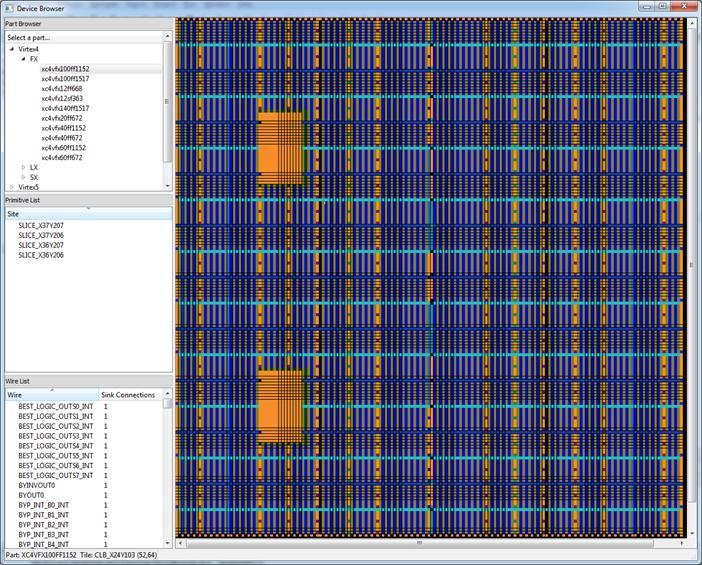
\includegraphics[width=0.8\columnwidth]{deviceBrowser}
\caption{\pgm{DeviceBrowser} Sample Display}
\label{fig:deviceBrowser}
\end{figure}

\noindent This can be done either from within Eclipse or from the command line,
depending on how you are running RS2 (if running under OS X be sure to provide the
\opt{-XstartOnFirstThread JVM argument}.

If all goes well you should see a graphical representation showing the details
of a physical FPGA device as shown in \autoref{fig:deviceBrowser}.  You may
initially be zoomed far in and might want to zoom out to see the entire chip
layout.

\subsection{Device Files For Use With RS2}
Device files for one part (the {\em xc7a100tcsg324}) are included in the
distribution so you can immediately start working with RS2 using this part (initially, it
will be the only device available when you run the \pgm{DeviceBrowser} program
above).  The device files for this part can be found in the
\dir{\${RAPIDSMITH\_PATH}/devices/artix7} directory.               

If you desire to work with additional parts, follow the instructions found in the
file \fil{\$RAPIDSMITH\_PATH/doc/InstallingNewDevices.txt}.

\section{Example RS2 Programs and Sample Vivado Designs}

A variety of example programs can be found in the
\pkg{edu.byu.edu.rapidSmith.examples} package in the RS2 installation.
They have been heavily commented and so provide a means to learn the RS2 API by
example as we believe this is much better than reading a lot of text trying to
teach you what you need to know.

There is a \fil{README.txt} file in that directory to provide an overview and
suggested order for learning from the examples.
In addition, the subsections below describe one or more built-in RS2 programs
which you might find useful.

\subsection{\pgm{DeviceBrowser}}
Note: this is a program from the original RapidSmith, but which is discussed
here because it is still very useful in RS2. 

This GUI program is located in \pkg{edu.byu.ece.rapidSmith.device.browser}
package.  It will let you browse parts at the tile level.  On the left, the user
may choose the desired part by navigating the tree menu and double-clicking on
the desired part name.  This will load the part in the viewer pane on the right
(the first available part is loaded at startup).  The status bar in the bottom
left displays which part is currently loaded.  Also displayed is the name of the
current tile which the mouse is over, highlighted by a yellow outline in the
viewer pane. The user may navigate inside the viewer pane by using the mouse.
 By right-clicking and dragging the cursor, the user may pan.  By using the
scroll-wheel on the mouse, the user may zoom.  If a scroll-wheel is unavailable,
the user may zoom by clicking inside the viewer pane and pressing the minus(-)
key to zoom out or the equals(=) key to zoom in.

All that is required for this to operate is a valid device file (no design
required). A screenshot of the \pgm{DeviceBrowser} program is shown in
\autoref{fig:deviceBrowser}.

\begin{figure}[htb]
\centering
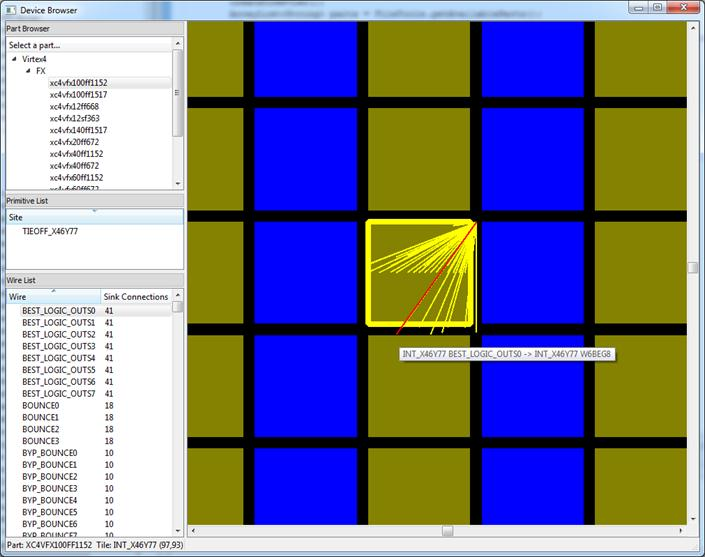
\includegraphics[width=0.8\columnwidth]{deviceBrowser2}
\caption{\pgm{DeviceBrowser} Screen Shot Showing Wire Connections}
\label{fig:deviceBrowser2}
\end{figure}

The device browser also allows the user to follow the various connections found
in the FPGA.  By double clicking a wire in the wire list, the application will
draw the connection on the tile array (as shown in the screenshot below).  By
hovering the mouse pointer over the connection, the wire becomes red and a
tooltip will appear describing the connection made by declaring the source tile
and wire followed by an arrow and the destination tile and wire.  By
clicking on the wire, the application will redraw all the connections that can
be made from the currently selected wire.  By repeating this action, the user
can follow connections and discover how the FPGA interconnect is laid out.  This
is shown in \autoref{fig:deviceBrowser2}.  Thanks to Chris Lavin for originally
creating this app.

\subsection{The \pgm{DesignAnalyzer} Test Program}
This program, along with a number of other example programs, is located in the\\
\pkg{edu.byu.ece.rapidSmith.examples} package.  After loading a design from a
checkpoint, it simply walks the design data structure, printing out what it
finds as it goes.  As such, it provides a nice example of a number of things
which would be useful for getting started with RS2:
\begin{itemize}
  \item How to enumerate the Cells in a design, determine and print their 
  placement information as well as their properties.
  \item How to enumerate the logical nets in a design and print out their source
  and sink pins. 
  \item How to traverse and print out the physical route for a logical net (if
  it is routed)  
\end{itemize}

\subsection{The \pgm{DeviceAnalyzer} Test Program}
This program is also located in the \pkg{edu.byu.ece.rapidSmith.examples}
package.  It is designed as a simple getting started program and demonstrates
how to query and print tiles in a device, wires in a tile, etc.

\subsection{Other Test Programs}
See the README.txt file in the \pkg{edu.byu.ece.rapidSmith.examples} package
directory.  It outlines the other test programs there which may be useful in
coming up to speed on RS2. 

\subsection{Sample Vivado Designs}
To enable new users of RS2 to be able to quickly start running the above test
programs, a small set of pre-compiled Vivado designs have been included in the
RS2 distribution.  They are located in the \dir{exampleVivadoDesigns} directory
and consist of 3 designs: 
\begin{itemize}
\item \sbr{add}: synthesized only
\item \sbr{cordic}: synthesized and placed
\item \sbr{count16}: synthesized, placed and routed
\end{itemize} 
The RS2 checkpoints are contained in
the following directories: \dir{add.tcp}, \dir{cordic.tcp}, and
\dir{count16.tcp}.
Vivado checkpoints are also included and are the \fil{add.dcp},
\fil{cordic.dcp}, and \fil{count16.dcp} files.  

To re-build one of the example designs in Vivado a compile script called
\pgm{compile.tcl} has been included in the \dir{exampleVivadoDesigns}
directory.  To re-build one of the sample designs, you would start up the Vivado
Tcl shell from your Vivado distribution and then execute the following in the Tcl shell:                
\vspace{-0.15in}  \begin{code}
	\% cd <path to exampleVivadoDesigns directory>
	\% compile_hdl_to_checkpoint_files add
	\% close_project
\end{code}
This will re-synthesize, place, and route the add design and, from that compiled
design, generate the \dir{.tcp} directory and the \fil{.dcp} file.

\section{Designs in RS2}

Designs in RS2 are similar to the designs found in Vivado (and which are
exported as EDIF files from Vivado). 
They are essentially logical netlists.  They are represented and stored in the
data structures found in the \pkg{design.subsite} package.  A \cls{CellDesign}
consists of a collection of \cls{Cell} objects, interconnected by
\cls{CellNets}.
CellNets connect to the \cls{CellPins} on Cells.  CellNets typically have one
source pin and one or more sink pins.  Cell objects have a name, properties, pins, a link to the library cell
they are an instantiation of, etc.

Cells may be placed onto \cls{BELs} and the corresponding CellPins mapped onto
\cls{BelPins}.  CellNets, when physically routed, map onto one or more
\cls{RouteTrees}.

\subsection{The Cell Class}
The example programs mentioned above provide examples of manipulating Cell
objects.  Here are a few things you should know about cells, in no particular
order: 
\begin{itemize}
\item A Cell always contains a reference to an object of type \cls{LibraryCell},
which serves as a template for its construction.
\item Cells may be physically  placed onto BELs in the device.  This is done by
setting the Cell's anchor value to point to the BEL it resides on.  If you know
where you want a Cell placed you can just place it there.  On the other hand,
RS2 provides a way to identify the Site/BEL combinations where a Cell could be
placed.  See the program \pgm{CreateDesignExample} in the \dir{examples}
directory for an illustration of how to do it both ways.
\item Cell objects have pins on their periphery where CellNets connect to.
\item The top-level ports of a design are tied to \cls{IPORT}, \cls{OPORT}, or
\cls{IOPORT} Cell objects.  These are pseudo-cells (you won't find them in
Vivado) and represent the terminal points for signals leaving or entering the top-level.  
\end{itemize}

\subsubsection{Cell Properties}
Cells as represented in EDIF files coming from Vivado may contain properties. 
For example, a D flip flop cell (FDRE) has a \env{CONFIG.INIT} property,
indicating what its power-up state should be.  These properties can be set to modify the
Cell's behavior.  The \pgm{DesignAnalyzer} test program described above
pretty-prints an RS2 logical design and, as a part of its operation, it lists the properties
set on each Cell in the design.  Here are some additional things about
properties you should know:
\begin{itemize}
  \item	It might be of interest to learn what properties could be set
  for a given cell.  This set of properties can be found in the
  \fil{cellLibrary.xml} files generated for a given family (see the
  \dir{\$RAPIDSMITH\_PATH/devices} directory and its sub-directories to find
  these XML files for any devices installed). 
  The files are quite readable and from them you can learn much about the
  available LibraryCell types for a given FPGA family (look for the
  \cls{libcellproperty} tags in the file).  At some point in the future this
  information will be incorporated into the RS2 data structures so that user
  programs can query them and so RS2 can check whether they are legal values
  when set by a user program.   For now, user code can set properties and those
  will be exported into EDIF when going from RS2 back into Vivado.  However, no
  error checking will be done by RS2 as this is done.
  \item In a GUI view of devices in Vivado you will see polarity inverters in
  many sites allowing for programmable selection of a signal or its inverse. 
  This is shown in the GUI in the form of a 2:1 MUX.  The CLK signal
  and its inverse entering a SLICE is an example of this.  However, this is not
  explicitly represented in the device representation.  Rather, properties on
  the Cells driven by the mux output signals muxes indicate whether the signal
  is inverted or not.  For example, generate a 4-bit counter using rising-edge
  triggered flip flops in Vivado and generate an EDIF file for it.  You will see
  that the counter is constructed, in part from FDRE cells.  Now, modify the HDL
  for your counter to make it a falling-edge triggered counter and compare the
  resulting EDIF file.  The difference you will see is that the property on each
  of the FDRE cells called \env{CONFIG.IS\_C\_INVERTED} has been set, indicating
  it is a falling-edge triggered flip flop.  When \pgm{bitgen} is actually run
  by Vivado, the corresponding clock inverter will be programmed accordingly.
  \item It should go without saying that since there is only one such clock
  inverter in a SLICE, all the flip flops in a slice must be either rising-edge
  triggered or falling-edge triggered (they must have the same
  \env{CONFIG.IS\_C\_INVERTED} control set value).  If you violate this, Vivado
  will throw an error.  Similar restrictions exist for all cells in a site driven by
  shared programmable inverters.  For example, flip flops in a slice (FDRE
  LibraryCells) may share programmable inverters on their clock, clock enable,
  and R inputs.
\end{itemize}

\subsection{The CellNet Class}
\begin{itemize}
  \item	A CellNet has a type.  Legal values are WIRE, GND, VCC, and UNKNOWN. 
  The WIRE type is the one used for normal signals.  CellNets have one source
  pin and one or more sink pins (these are of type CellPin).  The CellNet class
  has methods for traversing these.
  \item	GND and VCC nets have some special characteristics. There is a single
  logical VCC net.  It is driven by a single RapidSmithGlobalVcc cell.  The
  output pin of that cell is the source of all VCC in the design. However,
  unlike other cells which get routed to, this cell is never physically placed. 
  The situation with GND is similar.
\end{itemize}

\subsubsection{Physical Routing of CellNets in RS2}
\begin{itemize}
  \item A CellNet is physically routed by determining the metal segments and
  intervening PIPs that are to be used to make up the route.  A physical net is
  called a \cls{Wire} and contains some number of RouteTree objects.  A given
  RouteTree object has the source of the route as its root and then branches
  represent the branching of the route between source and sink. The physical
  routing of a net is represented by attaching one or more RouteTree objects to
  the net.
  \item Normal wires (CellNets of type WIRE) have only one RouteTree, reflecting
  the fact that they have a single source and multiple sinks.  Note that a wire
  cannot be physical routed to the pin of a cell which has not yet been placed.
  \item Physically, GND and VCC nets are unique.  When a
  circuit has been routed by Vivado the result will be multiple physical VCC routes and multiple physical GND
  routes in the circuit.  Each route is represented by its own RouteTree object.
  The source for each of these RouteTree objects will be a wire which is
  connected to a TIEOFF.  These TIEOFFs are not physically placed but their
  locations can be inferred by the source wire for each of the RouteTrees making
  up the VCC or GND route.
  \item Once a CellNet's physical routing has been created as a RouteTree, that
  is converted to a directed routing string when RS2 designs are exported from
  RS2 back into Vivado.  The \pgm{DesignAnalyzer} program in the examples
  directory gives an example of tracing out the RouteTrees which represent a physically
  routed wire.                       
\end{itemize}
The program \pgm{DesignAnalyzer} in the \pkg{edu.byu.ece.rapidSmith.examples}
package provides an illustration of how to traverse a physically routed CellNet.  This
is done in its \sbr{createRoutingString()} method.  This method starts by
getting the RouteTree object associated with the source pin for the given CellNet.  It then
recursively follows the linked set of RouteTree objects to follow the wire. 
Liberal comments in the \pgm{DesignAnalyzer} program illustrate how this is
done.
Consult it for details.

\section{Devices in RS2}

\subsection{Devices in RS2}
A device is defined in RS2 as a unique Xilinx FPGA part that includes package
information but not speed grade (such as the {\em xc7a100tcsg324} device
included in the RS2 distribution).  Each device contains specific information concerning its
primitive sites, tiles, wires, IOBs, and PIPs that are available to realize
designs.  The device information is represented in RS2 in the device package. 
RS2 has significantly extended the original RapidSmith \cls{Device} class for
its use as well as how device files are generated.

A Device object consists of a collection of \cls{Tiles}, each of which contains
one or more \cls{Sites}.  A Site contains one or more \cls{Bels}.  Sites have
\cls{SitePins} around their periphery and Bel objects have \cls{BelPINs} around
theirs.

The physical wires in the device are represented by objects of type \cls{Wire},
\cls{TileWire}, and \cls{SiteWire}.  However, the goal of RS2 is to largely hide
the differences between these three wire object types and let the user simply deal
with \cls{Wire} objects.

The previously-mentioned \pgm{DeviceBrowser} and \pgm{DeviceAnalyzer} programs
illustrate how to load and browse a device down to the Tile and Wire levels.

\section{Routing in RS2}

\subsection{Wires and WireConnections}
Routing in RapidSmith is done using \cls{Wire} objects, which are described
in the devices section above. Wires are uniquely identified by their
corresponding tile and wire name (i.e. tile1/wire1), and are connected through
\cls{WireConnection} objects. There are two types of wire connections:

\begin {enumerate}
  \item \pgm{PIP Connections}: Connect two different wires through a
  Programmable Interconnect Point. Most PIP connections are found in
  switchbox tiles of an FPGA part (as shown in Figure \ref{fig:switchboxPIP}).
  These types of connections are important to FPGA routing, because they
  dynamically configure the routing network for a given design.
  
  \begin{figure}[H]
	\centering
	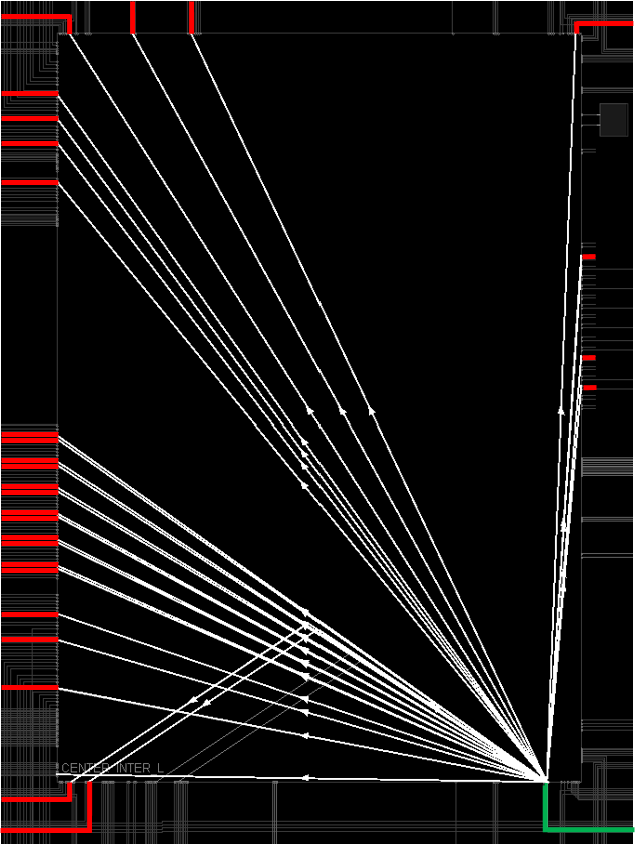
\includegraphics[width=0.8\columnwidth]{pipExample}
	\caption{An example of PIP wire connections in a device. The green wire
	represents the source wire, and the red wires represent all possible sink
	wires. In RapidSmith, the highlighed white sections of the
	figure are the PIP connections which can each be individually
	enabled or diabled.}
	\label{fig:switchboxPIP}
  \end{figure}
  
  \item \pgm{Non-PIP Connections}: Connect the same physical wire across two
  different tiles. In general, wires stretch across multiple tiles in a device, having
  a different name in each tile. This is demonstrated in figure
  \ref{fig:wireFigure}. The example wire shown in the figure spans 5
  different tiles, but has a different name in each. To save space, only the
  source and sink wire segments are kept in RapidSmith data structures
  (\texttt{INT\_X1Y1/E2BEG4}, \texttt{INT\_X2Y1/E2MID4}, and
  \texttt{INT\_X3Y1/E2END4}). The source segment is connected to each sink
  segment through a non-PIP wire connection.
\end{enumerate} 

\begin{figure}[H]
\centering
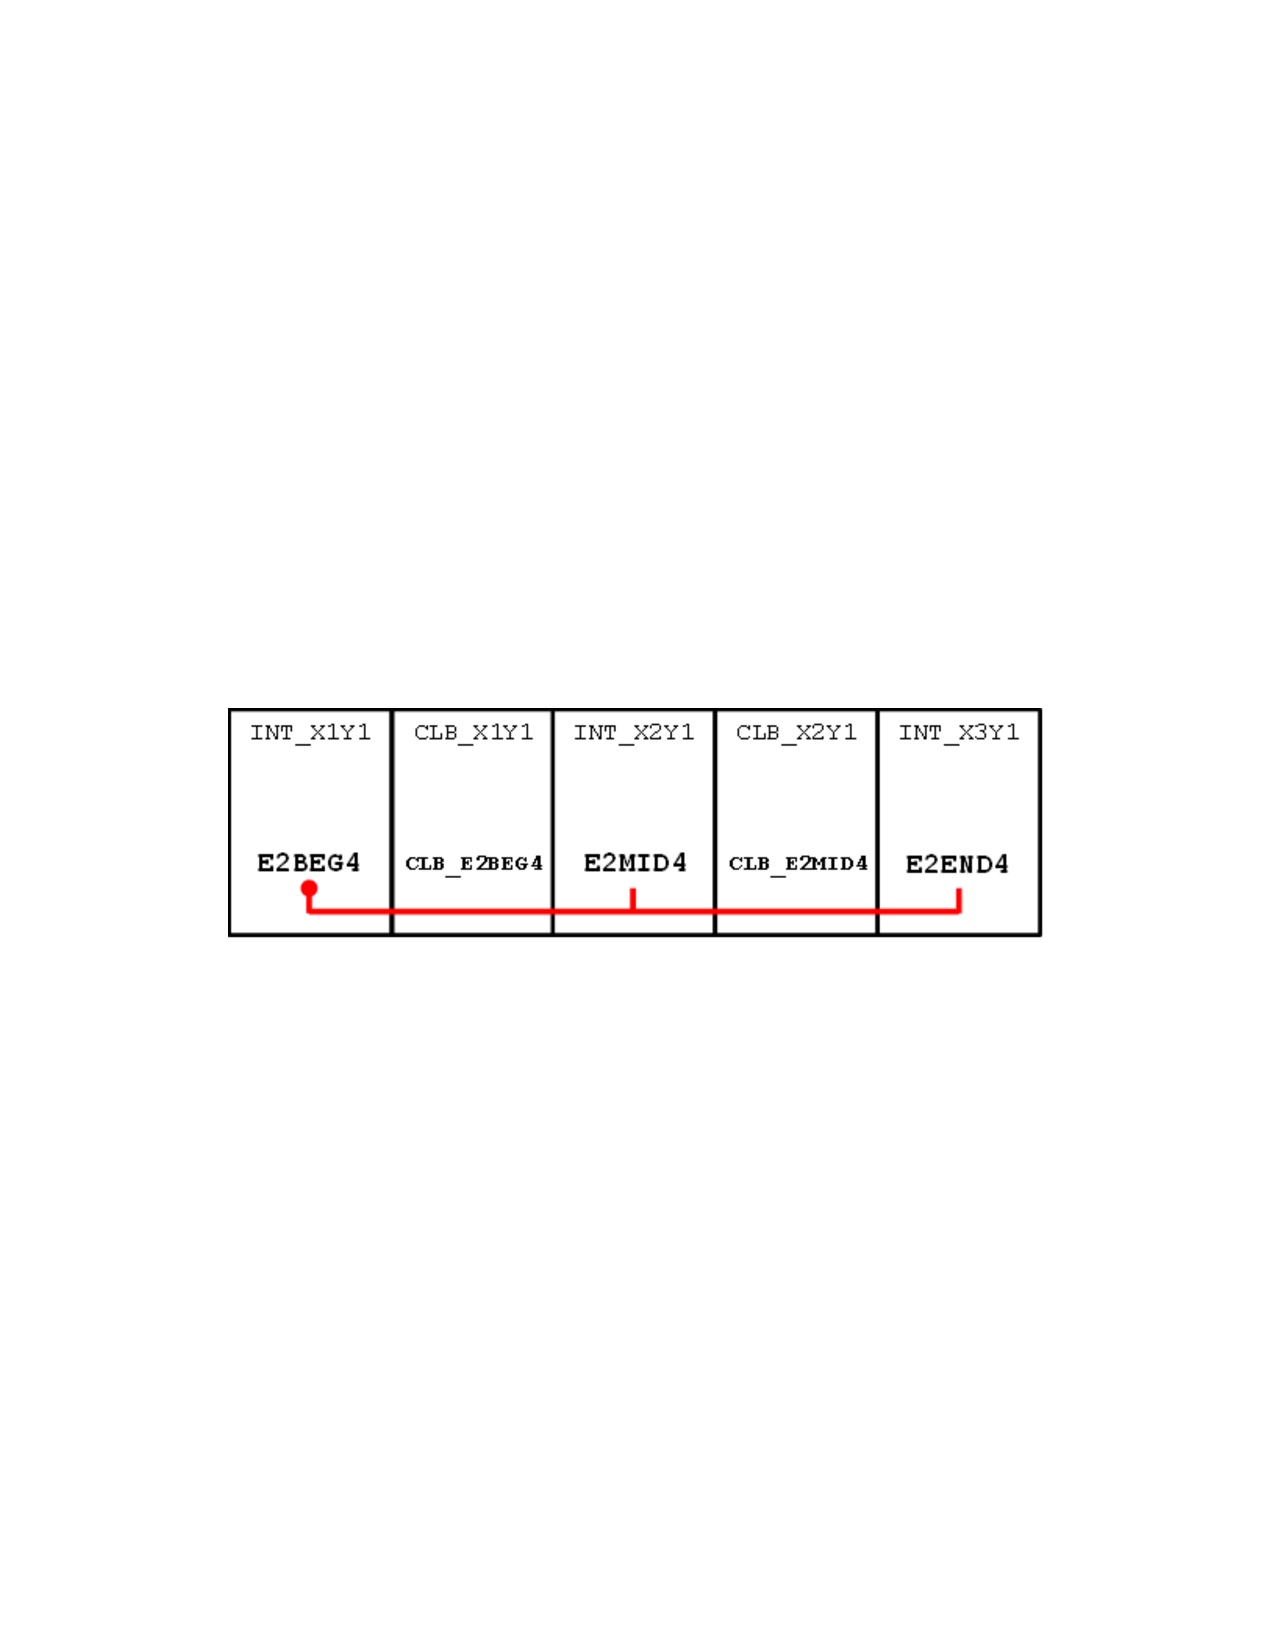
\includegraphics[width=0.8\columnwidth]{wireFigure}
\caption{A Wire in an FPGA Illustrating How Each Part of the Wire Has a
Different Name Depending on the Tile it is Located In}
\label{fig:wireFigure}
\end{figure}

\subsection{Traversing Wire Objects}
Traversing through wires in a device is straightforward. Given a handle to a
\cls{Wire} object named "mywire" or a \cls{WireConnection} object named
"wc", the following function calls can be used:

\begin {itemize}
  \item \texttt{mywire.getWireConnections()}: Returns a collection of all
  \cls{WireConnection}s with the source wire of mywire. This collection can be
  iterated through to find all places a specific wire goes (i.e. what wires it
  connects to).
  \item  \texttt{wc.isPip()}: Returns true if the wire connection ``wc'' is a PIP
  connection. Returns false otherwise.
  \item \texttt{wc.getSinkWire()}: Returns the sink wire of a wire connection.
\end{itemize} 

\noindent
In general, these are the only three functions that are needed to
search through the wires of a FPGA device. It is important to note however that
the first wire in the route has to be either (a) created using a \cls{TileWire}
constructor, or (b) retrieved from a function call of another object (such as
\texttt{SitePin::getExternalWire()}). To gain a better understanding of how to
use \cls{Wire}s and \cls{WireConnection}s, see the \pgm{HandRouter} example in
the RapidSmith repository.

\subsection{Other Types of Connections}
Along with PIP and non-PIP wire connections, there are several other types of
connections in RapidSmith. The source of the connection is always a \cls{Wire}
object, but the sink object differs. A description of these connections is found
below:

\begin {itemize}
  
  \item \pgm{Site Pin Connections}: Connects a \cls{Wire} to a \cls{SitePin}.
  The function call \texttt{conn.get\-SitePin()} can be used to get the sink
  \cls {SitePin} object.
  \item \pgm{Terminal Connections}: Connects a \cls{Wire} to a \cls{BelPin}. The
  function call \texttt{conn.get\-BelPin()} can be used to get the sink \cls
  {BelPin} object.
  \item \pgm{Site Routethrough Connections}: Connects an input site \cls{Wire}
  to an output site \cls{Wire}. A \cls{Site} in Vivado can be configured to pass
  the signal on an input \cls{SitePin} directly to an output \cls{SitePin}.
  These connections are represented as routethroughs in RapidSmith and can be
  determined with the function call \texttt{conn.isRoutethrough()}.
  \pgm{NOTE}: Before using this type of connection when building a
  routing data structure, make sure the \cls{Site} is unused.
  \item \pgm{BEL Routethrough Connections}: Connects an input BEL \cls{Wire} to
  an output BEL \cls{Wire}. Similarly to a \cls{Site} routethrough, LUTs in
  Vivado can also be configured as routethroughs. In this case, the signal on one of the
  input pins of the LUT is passed directly to the output pin of the LUT. A BEL
  routethrough connection can be used to configure a LUT as a routethrough in
  RapidSmith.
  \pgm{NOTE}: Before using this type of connection, make sure the LUT is
  unused (i.e. no cell is placed on it).
\end{itemize}

\noindent
When traversing through the device data structure, a generic \cls{Connection}
object is usually used. This connection can refer to any of the connections
described so far in this documentation.

\subsection{RouteTrees}

\cls{Wire}s and \cls{WireConnection}s are the fundamental objects used to
specify and explore routing in RapidSmith, but they need to be encapsulated in
a higher-level data structure to give meaning to the route of a \cls{CellNet}.
In the original RapidSmith, creating this data structure was up to the user.
RapidSmith 2 introduces the \cls{RouteTree} data structure, which handles
\cls{Wire}s, \cls{WireConnection}s, and branching while routing a
\cls{CellNet}. As figure \ref{fig:routeTree} shows, it is a simple tree
structure that organizes wires and wire connections. The fields in
a \cls{RouteTree} include:

\begin{itemize}
  \item A link to the the parent \cls{RouteTree}
  \item The \cls{Connection} from the parent tree to the current tree
  \item A list of sink \cls{RouteTree} children
  \item A cost field for routers 
\end{itemize}

\noindent
When a design is imported from Vivado, the routing information is representated
using \cls{Route\-Tree}s. On design export, the \cls{RouteTree} for each
\cls{CellNet} is parsed and converted into a Vivado ROUTE string. A user can use
custom data structures to route a design, but it needs to be
converted to an equivalent RouteTree data structure before exporting the
design to Vivado. The \pgm{DesignAnalyzer} example demonstrates how to
iterate through a \cls{RouteTree}. The \pgm{AStarRouter} and \pgm{HandRouter}
examples demonstrate how to build a \cls{RouteTree}.

\begin{figure}[H]
\centering
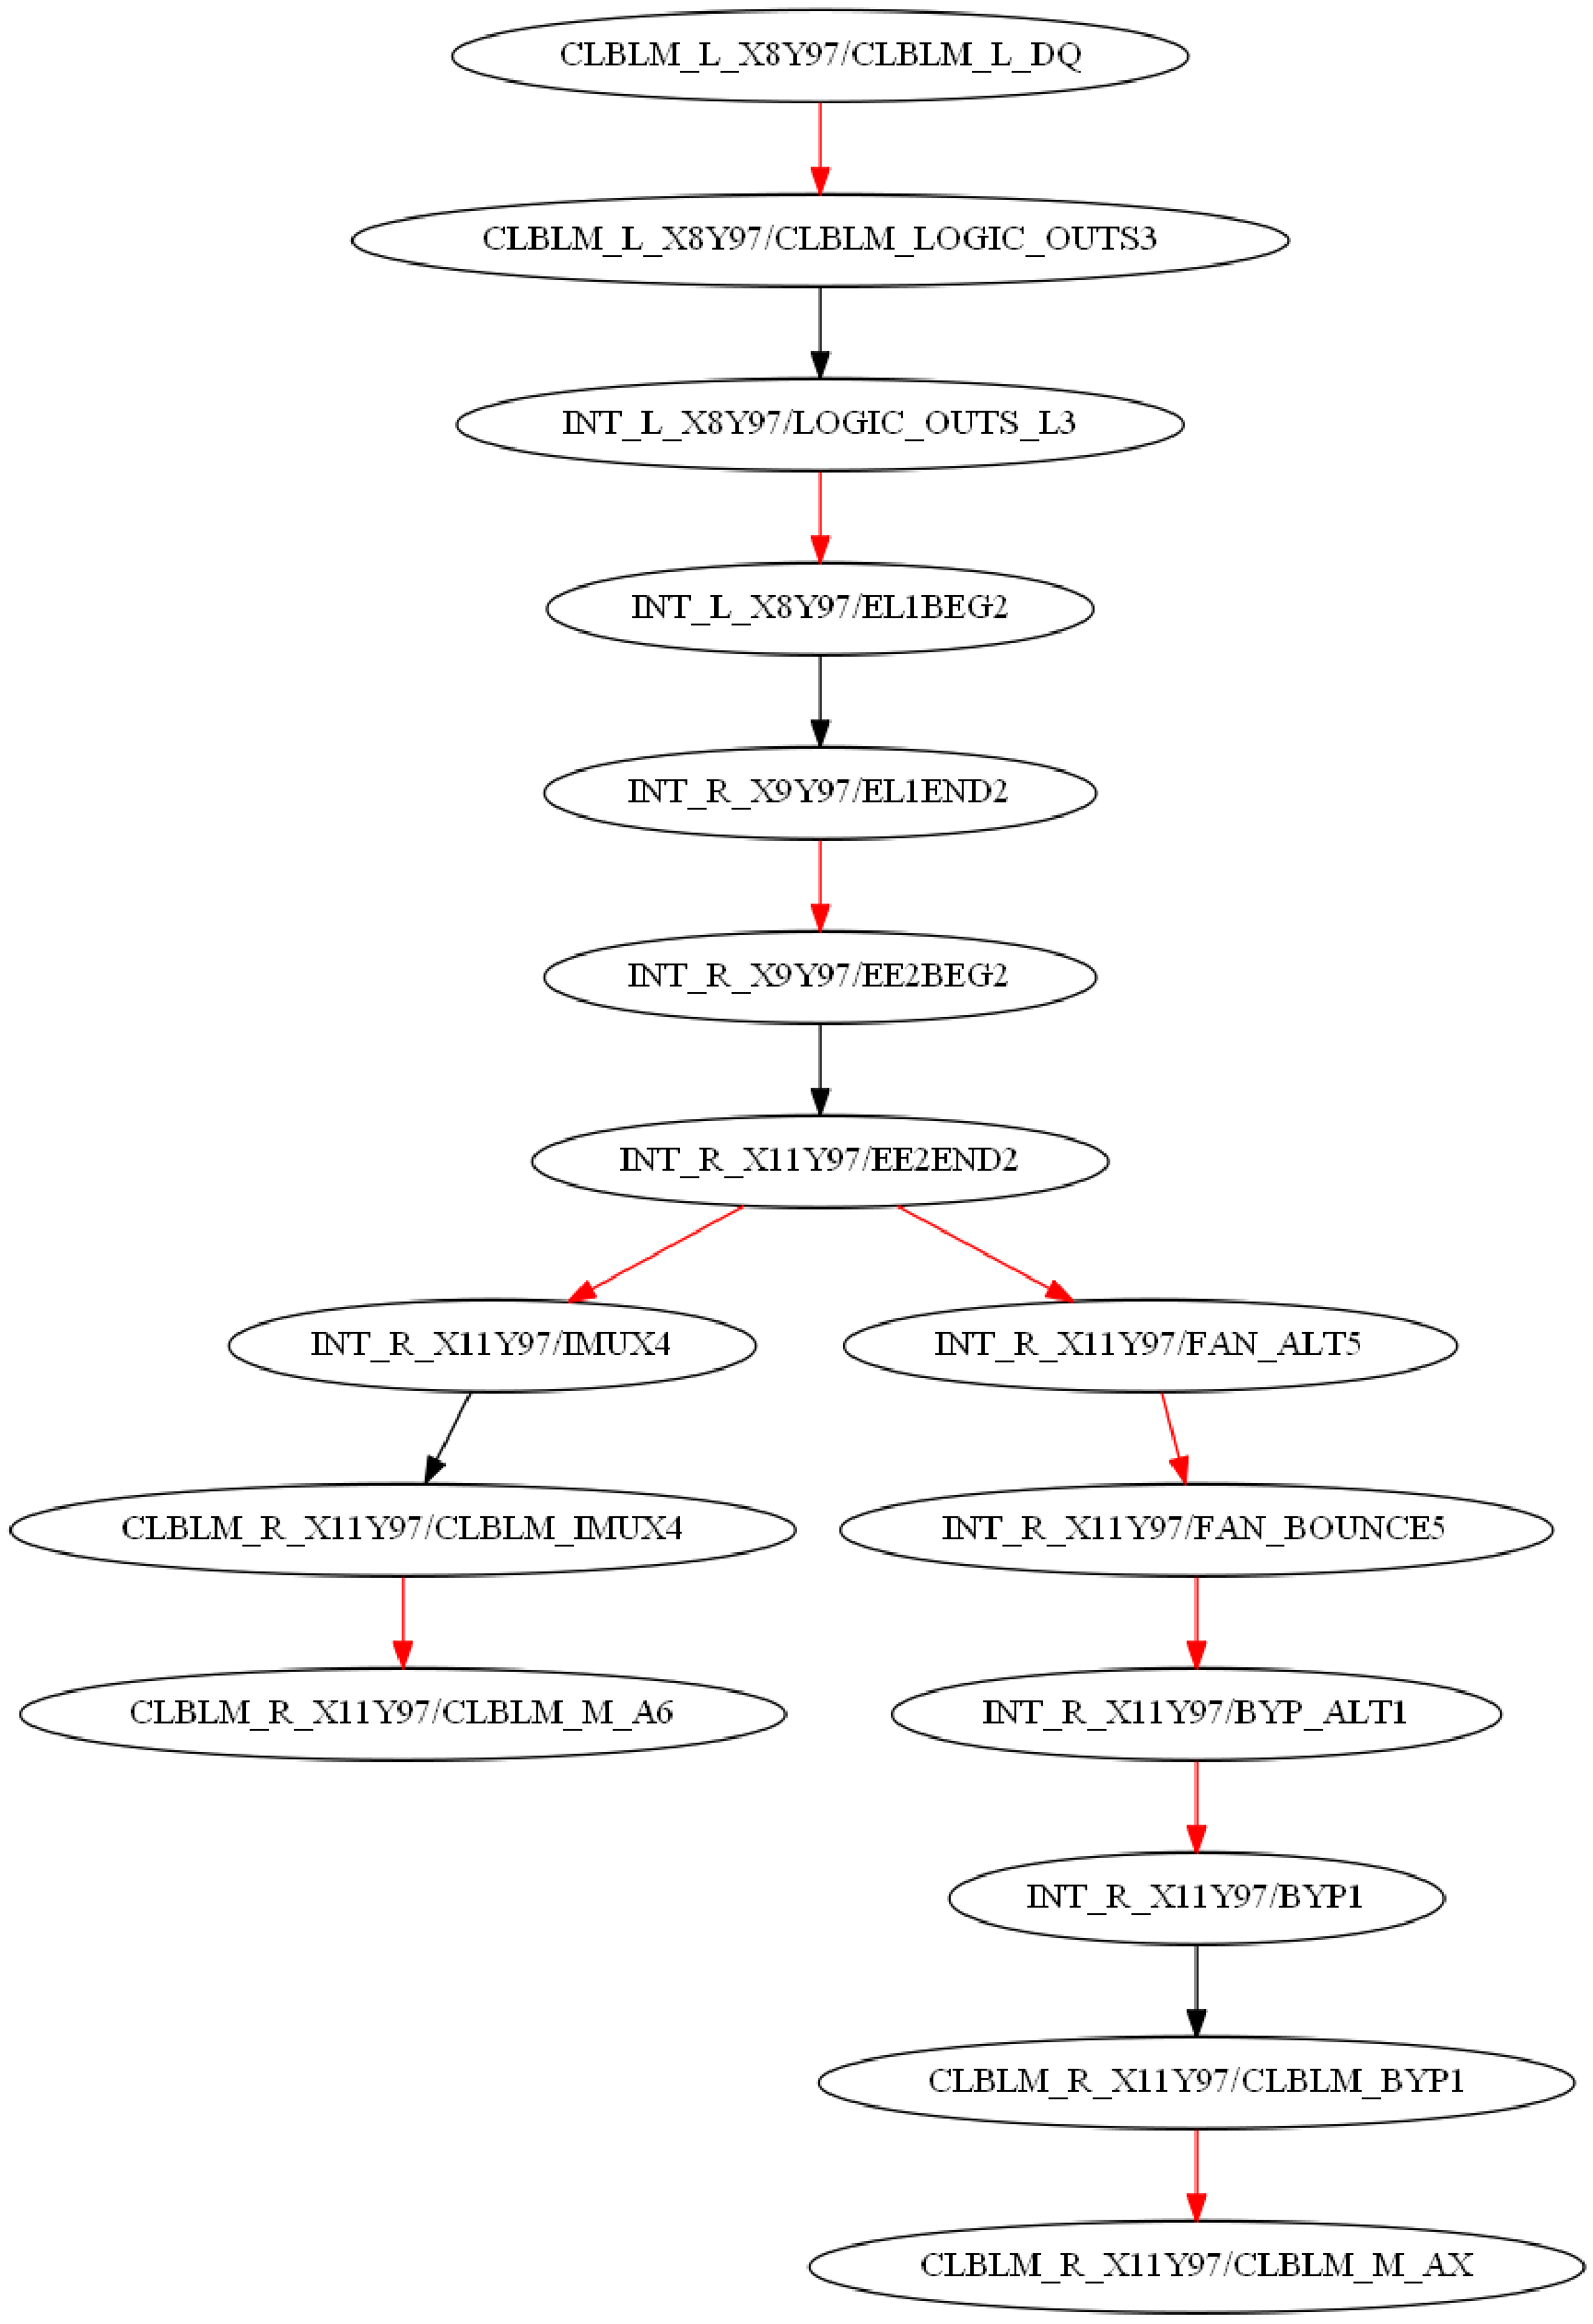
\includegraphics[width=0.8\columnwidth]{routeTree}
\caption{A DOT file representation of the RapidSmith2 RouteTree data structure.
Red edges represent PIP wire connections, and black edges represent non-PIP
wire connections. This specific RouteTree was created from the \pgm{AStarRouter}
example.}
\label{fig:routeTree}
\end{figure}


\section{Importing/Exporting Designs Between Vivado and RS2}

Importing and export designs between Vivado and RS2 is straightforward.  See the
program edu.byu.ece.rapidSmith.examples.ImportExportExample for an illustration
of how to do this.

\section{Bitstreams in RS2}

In the original RapidSmith, bitstreams can be parsed, manipulated, and exported
for Virtex 4, Virtex 5 and Virtex 6 Xilinx FPGA families.  Because of the
proprietary nature of Xilinx bitstreams, RapidSmith provided only documented
functionality when working with bitstreams (and was limited mainly to
manipulation at the frame level including helping to assemble sequences of
configuration commands which are interpreted by the FPGA configuration
controller circuitry).  While this has proven valuable to many researchers, it
does not provide the ability to create your own bitstream from scratch because
it does not provide the specific meaning of each bit in a bitstream.

If you desire to use RapidSmith's bitstream manipulation features, you should
download and work with RapidSmith instead of RS2 (the RapidSmith bitstream
packages have been removed from RS2).  If you do so, note that RapidSmith's
bitstream packages have not been tested beyond Virtex 6.  The authors would be
interested in upgrading RapidSmith's bitstream functionality to device families
beyond Virtex 6 if users create it and are willing to contribute it to us for
inclusion.

\section{Legal and Dependencies}
RS2 is released under GPL version 3.

\subsection{RapidSmith Legal Text}
\begin{quotation}
   BYU RapidSmith Tools

   Copyright (c) 2010-2016 Brigham Young University
   
   BYU RapidSmith Tools is free software: you may redistribute it
   and/or modify it under the terms of the GNU General Public License
   as published by the Free Software Foundation, either version 2 of
   the License, or (at your option) any later version.
   
   BYU RapidSmith Tools is distributed in the hope that it will be
   useful, but WITHOUT ANY WARRANTY; without even the implied warranty
   of MERCHANTABILITY or FITNESS FOR A PARTICULAR PURPOSE. See the GNU
   General Public License for more details.
   
   A copy of the GNU General Public License is included with the BYU
   RapidSmith Tools. It can be found at doc/gpl2.txt. You may also get
   a copy of the license at \url{http://www.gnu.org/licenses/}.
\end{quotation}

\section{Included Dependency Projects}
RS2 includes the Caucho Technology Hessian implementation which is distributed
under the Apache License. A copy of this license is included in the doc
directory in the file APACHE2-LICENSE.txt. This license is also available for
download at: \url{http://www.apache.org/licenses/LICENSE-2.0}. 

The source for the Caucho Technology Hessian implementation is available at:
\url{http://hessian.caucho.com}.

RS2 also includes the Qt Jambi project jars for Windows, Linux and Mac OS X.  Qt
Jambi is distributed under the LGPL GPL3 license and copies of this license and
exception are also available in the /doc directory in files LICENSE.GPL3.TXT and
LICENSE.LGPL.TXT respectively. These licenses can also be downloaded at:
\url{http://www.gnu.org/licenses/licenses.html}.
   
Source for the Qt Jambi project is available at:
\url{http://qt.nokia.com/downloads} and more recent versions are available at:
\url{http:/qt.gitorious.org/qt-jambi}.

RS2 also includes the JOpt Simple option parser which is released under
the open source MIT License which can be found in this directory in the file
MIT\_LICENSE.TXT.  A copy of this license can also be found at:
\url{http://www.opensource.org/licenses/mit-license.php}.
   
A copy of the source for JOpt Simple can also be downloaded at:
\url{http://jopt-simple.sourceforge.net/download.html}.

RS2 also includes the JDOM jars.  JDOM is available under an Apache-style open
source license, with the acknowledgment clause removed. This license is among
the least restrictive license available, enabling developers to use JDOM in
creating new products without requiring them to release their own products as
open source. This is the license model used by the Apache Project, which created
the Apache server. The license is available at the top of every source file and
in LICENSE.txt in the root of the JDOM distribution.                

The user is responsible for providing copies of these licenses and making
available the source code of these projects when redistributing these jars.

\section{Appendix}
TBD


\end{document}


%%% Local Variables: 
%%% mode: latex
%%% TeX-master: "main"
%%% End: 
